% !TeX root = ../main.tex

\chapter{Resultados}



  \section{Requerimientos}

  En esta sección se presentan los artefactos generados durante la fase de inicio del proyecto siguiendo la metodología propuesta. Estos artefactos son una primera versión de lo que se fue iterando durante el desarrollo de las actividades definidas.\\
  A continuación, se detallan las historias de usuario (HU) que definen los requerimientos funcionales, así como la matriz de riesgos que identifica y evalúa los posibles obstáculos que podría haber afectado el desarrollo del videojuego serio.



  \subsection{Historias de Usuario}


  Se empezó escribiendo la HU en base a las ideas principales y las mecánicas básicas, después se empezó modificar y/o crear ciertas HU dirigidos a cumplir con los aspectos escenciales para considerar el videojuego como un GBL.\\
  La primera iteración de las HU se redactaron en una tabla simple que contenía únicamente el código y la descripción de cada historia.
  Esta versión inicial sirvió como base para identificar las funcionalidades clave del sistema y establecer un marco de referencia para el desarrollo posterior.
  La Tabla \ref{tab:hu-inicial} muestra las historias de usuario definidas en la primera iteración.

\begin{longtable}{|c|L{12cm}|}
\caption{Primera versión de las Historias de Usuario} \label{tab:hu-inicial} \\
\hline
\textbf{Código} & \textbf{Historia de Usuario} \\ \hline
\endfirsthead

\hline
\textbf{Código} & \textbf{Historia de Usuario} \\ \hline
\endhead

\hline
\multicolumn{2}{r}{\textit{Continúa en la siguiente página}} \\
\endfoot

\hline
\endlastfoot
HU1 & Como jugador, quiero ver una pantalla de selección de niveles para elegir cuál jugar  \\ \hline
HU2 & Como jugador, quiero que al empezar un nivel, se me presente una pantalla de contrato que detalle el presupuesto, los objetivos y los posibles desafíos \\ \hline
HU3 & Como jugador, quiero poder mover la cámara (panorámica) por el mapa para explorar el terreno \\ \hline
HU4 & Como jugador, quiero poder acercar y alejar la vista (zoom) para ver el mapa con diferentes niveles de detalle \\ \hline
HU5 & Como jugador, quiero ver las delimitaciones políticas y ríos \\ \hline
HU6 & Como jugador, quiero ver un terreno del nivel a jugar \\ \hline
HU7 & Como jugador, quiero poder rotar la cámara para observar el terreno desde distintos ángulos \\ \hline
HU8 & Como jugador, quiero poder activar una capa de eventos para visualizar las zonas de riesgo y planificar mi ruta en consecuencia \\ \hline
HU9 & Como jugador, quiero poder construir un tramo de vía férrea entre dos puntos \\ \hline
HU10 & Como jugador, quiero poder eliminar un tramo de vía férrea para rediseñar mis rutas \\ \hline
HU11 & Como jugador, quiero que se pueda construya un puente o valles \\ \hline
HU12 & Como jugador, quiero que se construya automáticamente un túnel si mi vía férrea atraviesa una montaña \\ \hline
HU13 & Como jugador, quiero poder construir estaciones en puntos específicos de la vía para definir los puntos de inicio y fin del ciclo \\ \hline
HU14 & Como jugador, quiero que la interfaz muestre mi presupuesto actual en todo momento para controlar mis gastos de construcción \\ \hline
HU15 & Como jugador, quiero poder deshacer mi última acción de construcción para corregir un error rápidamente \\ \hline
HU16 & Como jugador, tras diseñar la ruta, quiero acceder a un menú para seleccionar y comprar la locomotora que usaré \\ \hline
HU17 & Como jugador, quiero poder añadir vagones específicos (pasajeros, carga) a mi locomotora para cumplir los requisitos del contrato \\ \hline
HU18 & Como jugador, quiero que el menú de selección me muestre las locomotoras de la ruta que diseñé \\ \hline
HU19 & Como jugador, durante la simulación, quiero ver una alerta o efecto visual cuando un tren está sufriendo daños al pasar por una zona de evento \\ \hline
HU20 & Como jugador, quiero que el botón de "Hacer Testeo" me informe si me falta algún requisito para iniciar la simulación \\ \hline
HU21 & Como jugador, quiero tener la opción de volver a la fase de construcción después de un testeo para modificar mis rutas antes de la evaluación final \\ \hline
HU22 & Como jugador, al finalizar un nivel, quiero ver una pantalla de puntuación que califique mi desempeño \\ \hline
HU23 & Como jugador, quiero que mi puntuación final considere la rentabilidad (costo total vs. valor del contrato) \\ \hline
HU24 & Como jugador, quiero que mi puntuación final considere la durabilidad (estado final de mis trenes y vías tras la simulación) \\ \hline
HU25 & Como jugador, quiero que mi puntuación final considere la eficiencia (tiempo que tardó el tren en completar el ciclo) \\ \hline
HU26 & Como jugador, quiero ver un informe detallado que desglose mi puntuación final para entender cómo mejorar \\ \hline
HU27 & Como jugador, quiero que se desbloqueen nuevos niveles en el menú de selección tras completar el contrato actual \\ \hline
HU28 & Como jugador, quiero que Don Raíl me presente el contrato al inicio de cada nivel con un diálogo breve, para darme un objetivo narrativo y contexto histórico sobre la región \\ \hline
HU29 & Como nuevo jugador, quiero que Don Raíl me guíe a través de un tutorial interactivo en el primer nivel, para aprender las mecánicas del juego de una forma amigable y contextual \\ \hline
HU30 & Como jugador, quiero que Don Raíl me dé una advertencia contextual si construyo una vía con una pendiente muy pronunciada o una curva muy cerrada, para que pueda corregir errores de ingeniería antes del testeo \\ \hline
HU31 & Como jugador, quiero que al seleccionar una estación o ciudad importante, aparezca un ícono de Don Raíl que pueda clickear para escuchar un dato histórico sobre la importancia ferroviaria de ese lugar \\ \hline
HU32 & Como jugador, quiero escuchar o leer un breve comentario de Don Raíl cuando un tren sufre un evento durante la simulación, para aumentar la inmersión \\ \hline
HU33 & Como jugador, quiero que Don Raíl comente sobre mi puntuación final, celebrando el éxito con emoción o dándome un consejo en caso de fallar para que la evaluación se sienta más personal \\ \hline
HU34 & Como jugador, quiero que durante las pantallas de carga, aparezcan anécdotas cortas o "dichos" de Don Raíl sobre la vida en el ferrocarril, para enriquecer el mundo del juego y aprovechar los tiempos de espera \\ \hline
HU35 & Como administrador, quiero adquirir y guardar metadatos de los jugadores en una base de datos para poder generar informes \\ \hline
\end{longtable}

\section{Diseño}
% (Completar) vendria a ser elaboracion
% organizar las HU?
% explicar epicas tambien la tabla de epicas
\subsection{Organización de las HU}
Para organizar el desarrollo del proyecto, se definieron un conjunto de épicas que agrupan las principales funcionalidades del sistema.
Estas sirvieron como base para clasificar las historias de usuario y facilitar la planificación y el seguimiento del avance.
En la Cuadro \ref{tab:épicas} se presentan las épicas establecidas para el proyecto cada una enumerada para la futura agrupación de historias de usuario.
\begin{table}[H] \centering \caption{Épicas} \label{tab:épicas} 
\begin{tabular}{|c|l|} 
\hline \textbf{Épica} & \textbf{Nombre}\\ \hline 
1 & Selección de Nivel y Contratos \\ \hline 
2 & Interacción con el Mapa 3D \\ \hline 
3 & Sistema de Construcción de Vías \\ \hline 
4 & Gestión de Material Rodante \\ \hline 
5 & Motor de Simulación y Eventos \\ \hline 
6 & Sistema de Evaluación y Puntuación \\ \hline 
7 & Progresión y Rejugabilidad \\ \hline 
8 & Narrativa y Mentoría\\ \hline 
\end{tabular} 
\end{table}

Una vez definidas, se procedió a asignar cada épica a la historia de usuario correspondiente, de acuerdo con la funcionalidad o el componente 
del sistema al que contribuía. Esta clasificación permitió identificar con claridad el subsistema o área funcional a la que pertenecía cada historia, favoreciendo una organización más coherente del desarrollo y una mejor comprensión del alcance de cada módulo dentro del proyecto.
\begin{longtable}{|c|c|L{10cm}|}
\caption{Historias de Usuario} \label{tab:hu} \\
\hline
\textbf{Épica} & \textbf{Código} & \textbf{Historia de Usuario} \\ \hline
\endfirsthead

\hline
\textbf{Épica} & \textbf{Código} & \textbf{Historia de Usuario} \\ \hline
\endhead

\hline
\multicolumn{3}{r}{\textit{Continúa en la siguiente página}} \\
\endfoot

\hline
\endlastfoot
1 & HU1 & Como jugador, quiero ver una pantalla de selección de niveles para elegir cuál jugar  \\ \hline
1 & HU2 & Como jugador, quiero que al empezar un nivel, se me presente una pantalla de contrato que detalle el presupuesto, los objetivos y los posibles desafíos \\ \hline
2 & HU3 & Como jugador, quiero poder mover la cámara (panorámica) por el mapa para explorar el terreno \\ \hline
2 & HU4 & Como jugador, quiero poder acercar y alejar la vista (zoom) para ver el mapa con diferentes niveles de detalle \\ \hline
2 & HU5 & Como jugador, quiero ver las delimitaciones políticas y ríos \\ \hline
2 & HU6 & Como jugador, quiero ver un terreno del nivel a jugar \\ \hline
2 & HU7 & Como jugador, quiero poder rotar la cámara para observar el terreno desde distintos ángulos \\ \hline
2 & HU8 & Como jugador, quiero poder activar una capa de eventos para visualizar las zonas de riesgo y planificar mi ruta en consecuencia \\ \hline
3 & HU9 & Como jugador, quiero poder construir un tramo de vía férrea entre dos puntos \\ \hline
3 & HU10 & Como jugador, quiero poder eliminar un tramo de vía férrea para rediseñar mis rutas \\ \hline
3 & HU11 & Como jugador, quiero que se pueda construya un puente o valles \\ \hline
3 & HU12 & Como jugador, quiero que se construya automáticamente un túnel si mi vía férrea atraviesa una montaña \\ \hline
3 & HU13 & Como jugador, quiero poder construir estaciones en puntos específicos de la vía para definir los puntos de inicio y fin del ciclo \\ \hline
3 & HU14 & Como jugador, quiero que la interfaz muestre mi presupuesto actual en todo momento para controlar mis gastos de construcción \\ \hline
3 & HU15 & Como jugador, quiero poder deshacer mi última acción de construcción para corregir un error rápidamente \\ \hline
4 & HU16 & Como jugador, tras diseñar la ruta, quiero acceder a un menú para seleccionar y comprar la locomotora que usaré \\ \hline
4 & HU17 & Como jugador, quiero poder añadir vagones específicos (pasajeros, carga) a mi locomotora para cumplir los requisitos del contrato \\ \hline
4 & HU18 & Como jugador, quiero que el menú de selección me muestre las locomotoras de la ruta que diseñé \\ \hline
5 & HU19 & Como jugador, durante la simulación, quiero ver una alerta o efecto visual cuando un tren está sufriendo daños al pasar por una zona de evento \\ \hline
5 & HU20 & Como jugador, quiero que el botón de "Hacer Testeo" me informe si me falta algún requisito para iniciar la simulación \\ \hline
5 & HU21 & Como jugador, quiero tener la opción de volver a la fase de construcción después de un testeo para modificar mis rutas antes de la evaluación final \\ \hline
6 & HU22 & Como jugador, al finalizar un nivel, quiero ver una pantalla de puntuación que califique mi desempeño \\ \hline
6 & HU23 & Como jugador, quiero que mi puntuación final considere la rentabilidad (costo total vs. valor del contrato) \\ \hline
6 & HU24 & Como jugador, quiero que mi puntuación final considere la durabilidad (estado final de mis trenes y vías tras la simulación) \\ \hline
6 & HU25 & Como jugador, quiero que mi puntuación final considere la eficiencia (tiempo que tardó el tren en completar el ciclo) \\ \hline
6 & HU26 & Como jugador, quiero ver un informe detallado que desglose mi puntuación final para entender cómo mejorar \\ \hline
7 & HU27 & Como jugador, quiero que se desbloqueen nuevos niveles en el menú de selección tras completar el contrato actual \\ \hline
7 & HU28 & Como jugador, quiero que Don Raíl me presente el contrato al inicio de cada nivel con un diálogo breve, para darme un objetivo narrativo y contexto histórico sobre la región \\ \hline
8 & HU29 & Como nuevo jugador, quiero que Don Raíl me guíe a través de un tutorial interactivo en el primer nivel, para aprender las mecánicas del juego de una forma amigable y contextual \\ \hline
8 & HU30 & Como jugador, quiero que Don Raíl me dé una advertencia contextual si construyo una vía con una pendiente muy pronunciada o una curva muy cerrada, para que pueda corregir errores de ingeniería antes del testeo \\ \hline
8 & HU31 & Como jugador, quiero que al seleccionar una estación o ciudad importante, aparezca un ícono de Don Raíl que pueda clickear para escuchar un dato histórico sobre la importancia ferroviaria de ese lugar \\ \hline
8 & HU32 & Como jugador, quiero escuchar o leer un breve comentario de Don Raíl cuando un tren sufre un evento durante la simulación, para aumentar la inmersión \\ \hline
8 & HU33 & Como jugador, quiero que Don Raíl comente sobre mi puntuación final, celebrando el éxito con emoción o dándome un consejo en caso de fallar para que la evaluación se sienta más personal \\ \hline
8 & HU34 & Como jugador, quiero que durante las pantallas de carga, aparezcan anécdotas cortas o "dichos" de Don Raíl sobre la vida en el ferrocarril, para enriquecer el mundo del juego y aprovechar los tiempos de espera \\ \hline
6 & HU35 & Como administrador, quiero adquirir y guardar metadatos de los jugadores en una base de datos para poder generar informes \\ \hline
\end{longtable}

%colocar capturas de los primeros intentos
%capturas de los videos con explicaciones de que tanto se hacia y el como fue la adaptacion, entre esos mencionando el que el mapa antiguo estaba mal y porque y todo eso
\subsection{Elaboración de la maqueta}

\subsubsection{Terreno}
La primera maqueta a realizar se trataba del principal entorno de interacción que tendrá el jugador con el entorno, en este caso, el mapa en 3 dimensiones de Colombia.
Para eso, se realizó un modelado en \textit{Blender} utilizando una técnica de elevación por textura, en la cual se empleó una imagen en escala de grises para representar las variaciones de altura del terreno (DEM).
Dicha imagen, de resolución limitada, permitió obtener un modelo base del relieve, aunque con una precisión reducida debido a la baja calidad del mapa de elevación.
En la Figura \ref{fig:mapa-altura} se presenta la textura empleada y el resultado del modelo tridimensional generado a partir de ella.
\begin{figure}[H]
\centering
\begin{minipage}{0.45\textwidth}
    \centering
    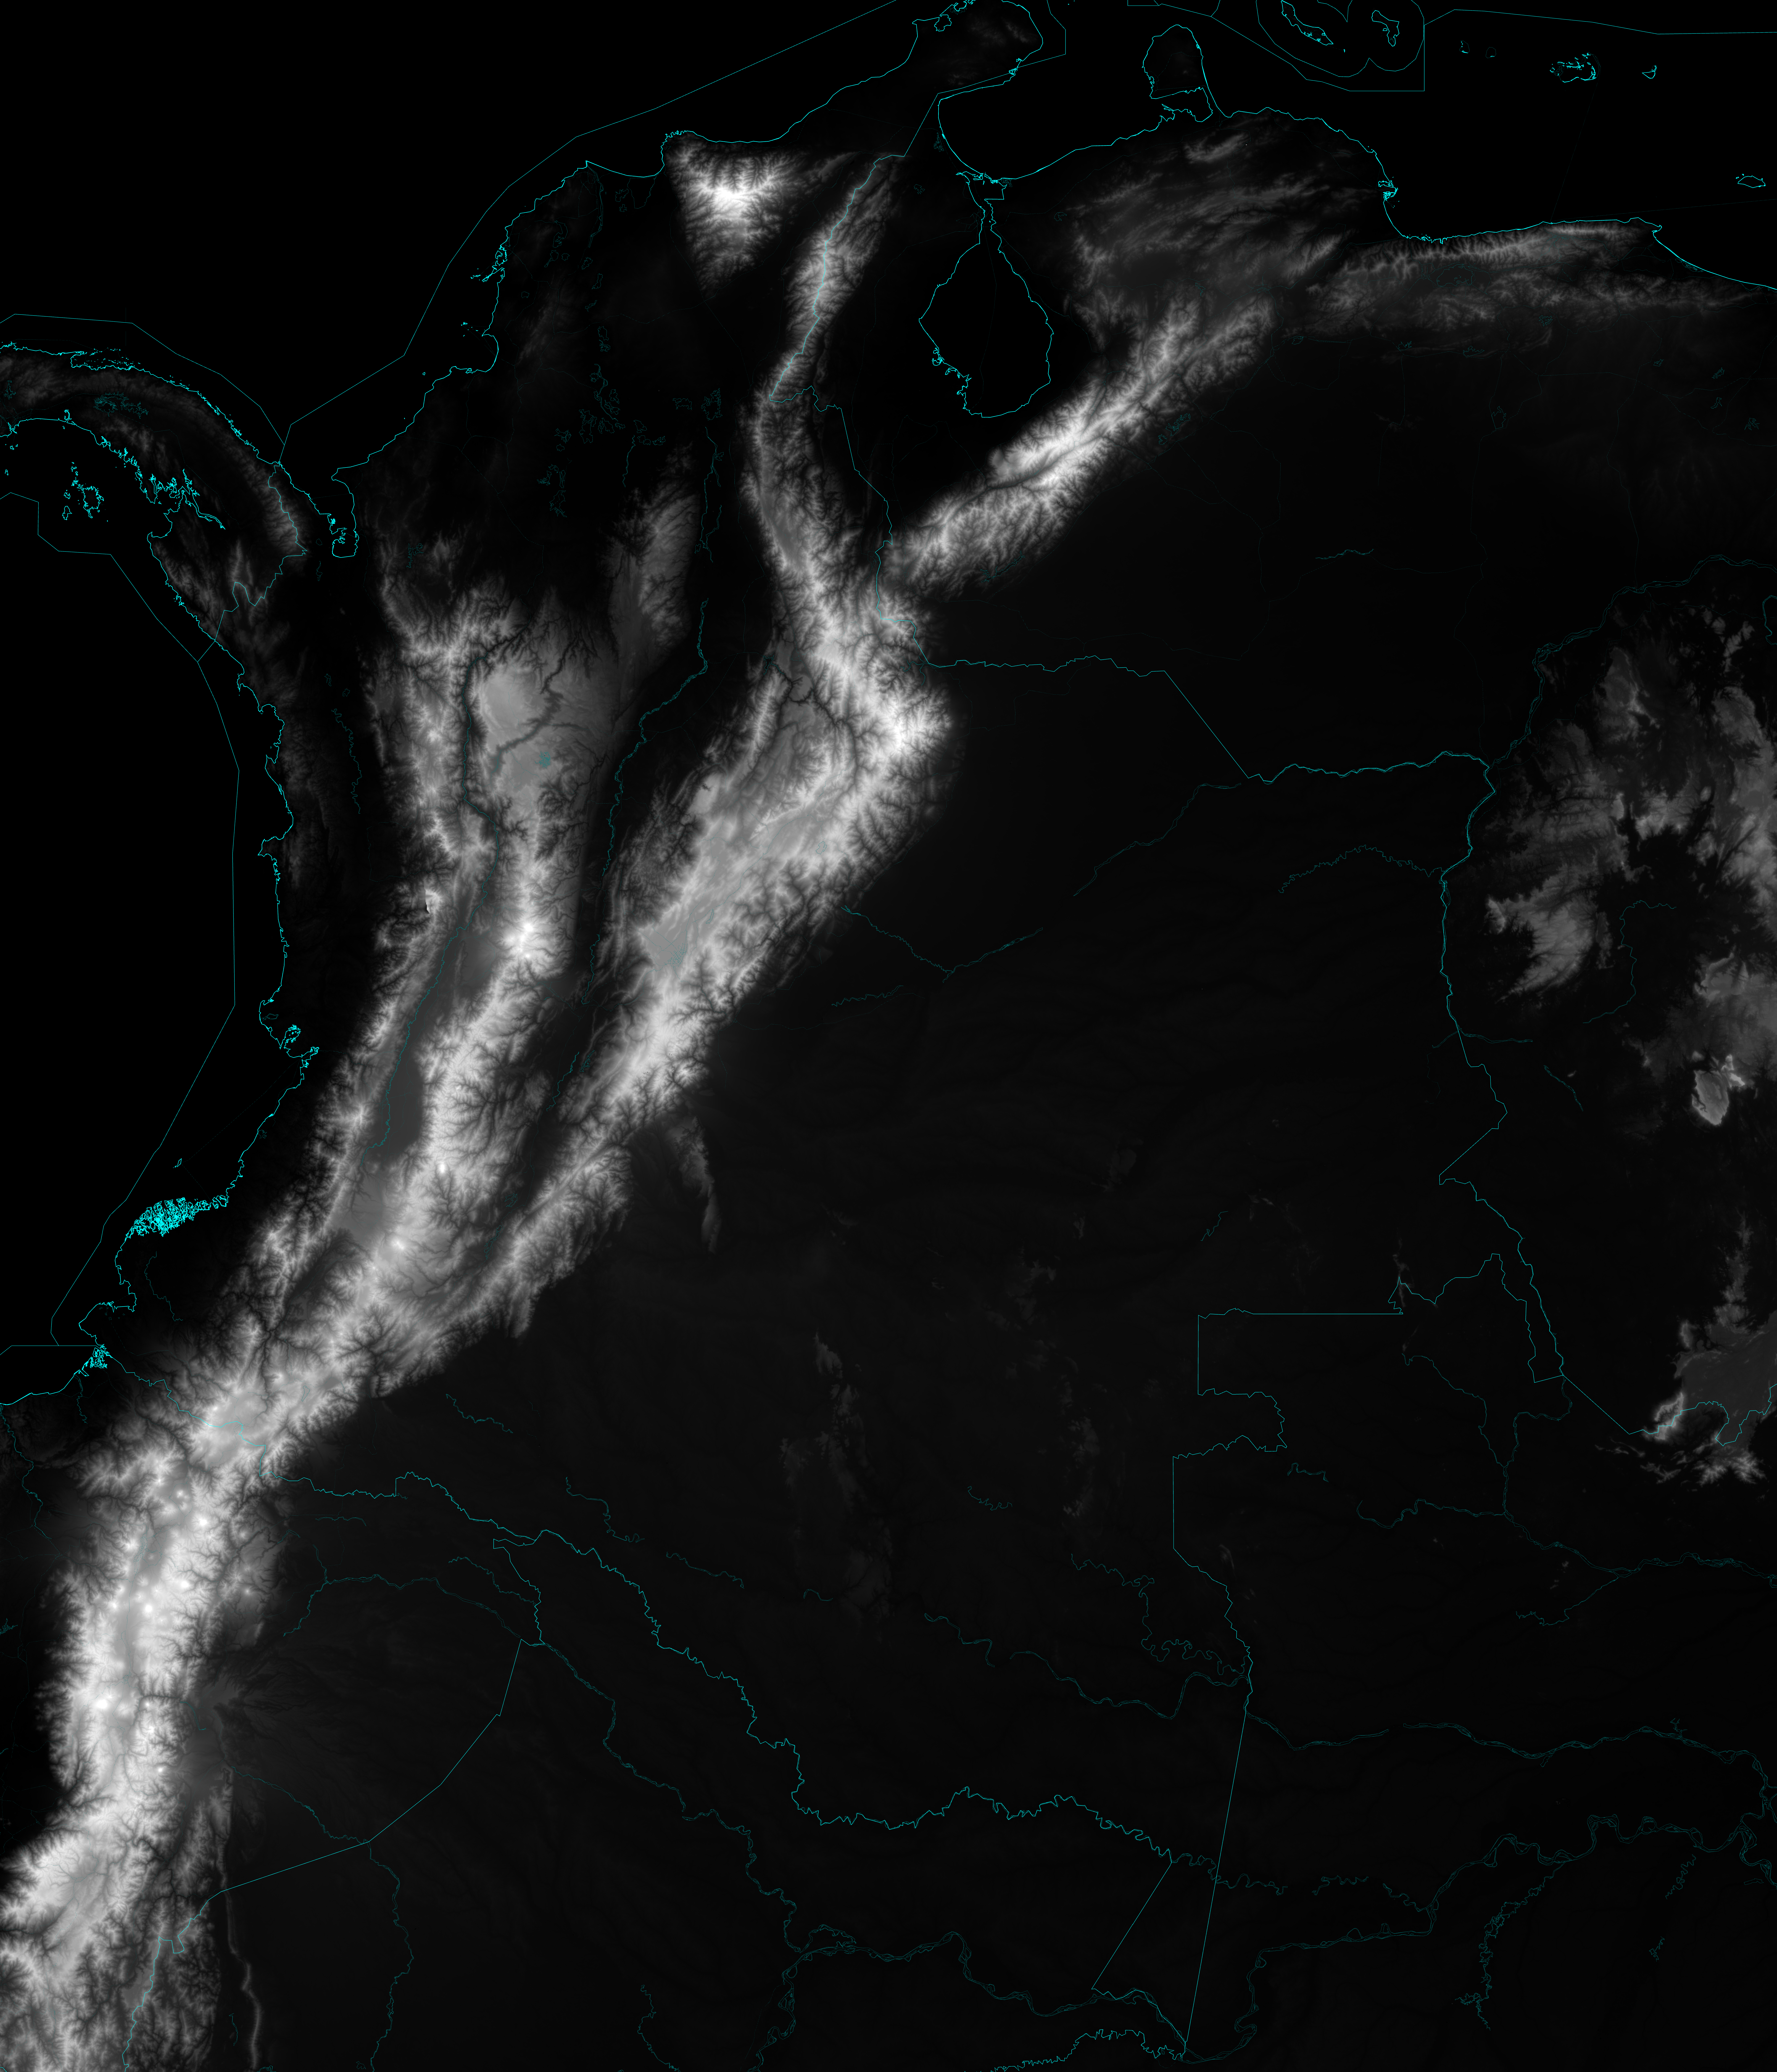
\includegraphics[width=\linewidth]{figures/mapa_alturas.png}
    \caption*{(a) Mapa de elevación en escala de grises.}
\end{minipage}\hfill
\begin{minipage}{0.45\textwidth}
    \centering
    \includegraphics[width=\linewidth]{figures/mapa_colombia_v1.jpeg}
    \caption*{(b) Modelo tridimensional generado en Blender.}
\end{minipage}
\caption{Generación del terreno mediante mapa de elevación en Blender.}
\label{fig:mapa-altura}
\end{figure}

Sin embargo, el modelo obtenido presentaba una alta densidad de polígonos, con un total de 24.5 millones de vértices, como se muestra en la Figura \ref{fig:rendimiento-terreno}.
Debido a ello, durante las pruebas se registró una tasa de cuadros por segundo (\textit{frames per second}, FPS) promedio de 25.9, valor considerablemente inferior al rango óptimo de 30 a 60 FPS recomendado para garantizar una experiencia fluida.
Este rendimiento reducido afectaba tanto el desempeño real del sistema como la percepción del usuario, generando una sensación de lentitud e inestabilidad en la simulación.
\begin{figure}[H]
\centering
\includegraphics[width=0.8\textwidth]{figures/bajo_rendimiento.jpeg}
\caption{Ejemplo del alto número de polígonos del modelo 3D que afecta el rendimiento.}
\label{fig:rendimiento-terreno}
\end{figure}

Esta situación evidenció que el uso de un modelo tridimensional completo para representar el terreno no era una solución óptima, especialmente considerando los requerimientos de eficiencia y fluidez del entorno de simulación.
Por ello, se decidió implementar un método alternativo, que anteriormente desconocíamos, de generación del mapa, con el fin de mejorar la eficiencia y el rendimiento general del entorno virtual.
\subsubsection{Vías}
En un intento por optimizar el proceso de generación del trazado ferroviario, se exploró inicialmente la posibilidad de representar las vías mediante la conexión de puntos y segmentos rectos.
Este enfoque, aunque sencillo en su concepción, requería una gran cantidad de puntos para lograr una precisión adecuada en curvas y pendientes, lo cual incrementaba la complejidad del sistema y afectaba el rendimiento general.
Ante esta limitación, se consideró el uso de \textit{splines}, una técnica matemática que permite la creación de curvas suaves a partir de un conjunto reducido de puntos de control.
Las splines resultan especialmente adecuadas para la representación de vías férreas, ya que facilitan la generación de trayectorias continuas y realistas sin necesidad de definir manualmente cada punto intermedio, mejorando así tanto la precisión geométrica como la eficiencia del proceso de renderizado.
%le añadimos las columnas a los riesgos, con una nueva *tabla de de que tanto riesgo hay* y con eso definimos la columna nivel de riesgo y pues se pone la tabla entera ahora si, lo hemos puesto abierto y cerrado si ya esta hecho
%que este cerrado es que ya se soluciono o se acepto, como los de poco riesgo, que puede..... osea existen cerrados que es porque el problema es muy minimo, no es tan grave

\subsection{Refinación de la lista de riesgos}

Para mejorar la comprensión y categorizar adecuadamente los posibles riesgos presentados en la sección \textit{PONER PRIMERA SECCIÓN DONDE SE 
PRESENTA EL DOC DE RIESGOS}, se diseñó un sistema de evaluación de riesgos compuesto por dos tablas complementarias.
En primer lugar, se definió un rango de niveles de riesgo, donde se definen los valores numéricos del 1 al 5 que representan la magnitud del impacto y la probabilidad de ocurrencia de un evento.
En esta escala, el valor 1 indica una afectación mínima o poco probable, mientras que el valor 5 corresponde a un evento con consecuencias críticas o de alta probabilidad, tal como se explica en la Figura \ref{fig:linea_impacto_probabilidad}.
\begin{figure}[H]\centering
  \includegraphics[width=\linewidth]{figures/linea de impacto-probabilidad.png}
  \caption{Rango de riesgos y Probabilidad.
Fuente: Propia}
  \label{fig:linea_impacto_probabilidad}
\end{figure}

En segundo lugar, se desarrolló una tabla general de riesgos, en la que se registran los posibles problemas identificados durante el proyecto.
Esta tabla incluye los campos Descripción (donde se detalla el problema detectado), Causa, Impacto, Probabilidad, Nivel de riesgo (calculado como el producto del impacto con la probabilidad), Plan de acción (estrategias o medidas a tomar) y Estado (donde se especifica si el riesgo permanece abierto o ya ha sido cerrado).
En la tabla \ref{tab:matriz-riesgos} se muestra el artefacto entregado.

Hay que aclarar que, algunos riesgos se mantuvieron abiertos incluso hasta el final del desarrollo del proyecto.
Esto se debe a que se consideró que el nivel de riesgo era suficientemente bajo como para evitar gastar recursos en solucionarlo.
\begin{landscape}
\begin{longtable}{|c|L{2.8cm}|L{2.8cm}|c|c|c|L{3.2cm}|c|}
\caption{Matriz de riesgos del proyecto}\label{tab:matriz-riesgos} \\
\hline
\multicolumn{1}{|c|}{\textbf{No. Ref}} &
\multicolumn{1}{c|}{\textbf{Descripción}} &
\multicolumn{1}{c|}{\textbf{Causa}} &
\multicolumn{1}{c|}{\textbf{Impacto}} &
\multicolumn{1}{c|}{\textbf{Probabilidad}} &
\multicolumn{1}{c|}{\textbf{Nivel de Riesgo}} &
\multicolumn{1}{c|}{\textbf{Plan de acción}} &
\multicolumn{1}{c|}{\textbf{Estado}} \\
\hline
\endfirsthead

\hline
\multicolumn{1}{|c|}{\textbf{No.
Ref}} &
\multicolumn{1}{c|}{\textbf{Descripción}} &
\multicolumn{1}{c|}{\textbf{Causa}} &
\multicolumn{1}{c|}{\textbf{Impacto}} &
\multicolumn{1}{c|}{\textbf{Probabilidad}} &
\multicolumn{1}{c|}{\textbf{Nivel de Riesgo}} &
\multicolumn{1}{c|}{\textbf{Plan de acción}} &
\multicolumn{1}{c|}{\textbf{Estado}} \\
\hline
\endhead

R1 & El modelo del terreno del mapa de Colombia está mal optimizado & El uso de modelo 3D genera una sobrecarga en la memoria gráfica & 4 & 4 & 16 & Realización de un terreno formal de Unity sin usar Blender.
Carga de terreno por bloques. & Cerrado \\ \hline
R2 & La cámara del jugador puede atravesar el terreno.
& La cámara no está programada para evadir o chocar con el mapa.
& 2 & 5 & 10 & Implementación de una función para aplicar una colisión de cámara con el terreno y evitar el paso.
& Abierto \\ \hline
R3 & Las vías se generan de manera poco natural e inconexa.
& Uso de puntos y rectas para la asignación de vías & 5 & 4 & 20 & Cambiar a uso de spline.
& Cerrado \\ \hline
R4 & Terreno con parches o incoherencias.
& El DEM utilizado está con ciertos datos erróneos o vacíos.
& 2 & 3 & 6 & Cambiar de DEM o arreglar los parches haciendo uso de algoritmos.
& Cerrado \\ \hline
R5 & Textura de vías solapando suelo en plano.
& Vía colocada en el punto exacto donde está el terreno, generando solapamiento & 1 & 2 & 2 & Mover las vías generadas una pequeña distancia hacia arriba & Cerrado \\ \hline
R6 & Las vías no permiten al tren dar vueltas en un circuito cerrado.
& Spline no cerrado & 2 & 3 & 6 & Añadir que el circuito detecte cuando se colocan vías cerca al punto inicial, y de ser así cierre el circuito & Cerrado \\ \hline
R7 & Dificultad para representar todos los ríos y lagos de Colombia en el mapa.
& Colombia tiene una gran densidad de elementos hidrológicos, que superan la capacidad de representación fiel en el terreno del videojuego.
& 4 & 4 & 16 & Definir criterios de selección: incluir solo ríos principales y lagos mayores.
& Abierto \\ \hline
R8 & Las vías atraviesan montañas & La generación de vías no interpola dichas alturas & 3 & 4 & 12 & Modificar la función de generación de vías, para que, cuando la vía atraviese el terreno, genere un túnel en la zona atravesada.
& Cerrado \\ \hline
R9 & Estadísticas de las locomotoras no son leídas correctamente & Estadísticas guardadas en los GameObject hijos de la Locomotora & 4 & 2 & 8 & Unificar la lógica y estadísticas de las distintas locomotoras en el GameObject padre Locomotora & Cerrado \\ \hline
R10 & HUD no muestra la vida actual del tren al hacer cambio de locomotora & Dato de vida y estadísticas no leído después del cambio & 2 & 2 & 4 & Crear una función para reiniciar las estadísticas del tren & Cerrado \\ \hline
R11 & Modelos 3D de los trenes y 
ciudades se ven a escalas diferentes & Escalas y rotaciones no aplicadas correctamente en Blender & 1 & 3 & 3 & Aplicar escalas y rotaciones a los modelos 3D de los trenes y ciudades & Cerrado \\ \hline
R12 & Shaders incompatibles y LOD's mal configurados.
& Unity tiene valores por defecto en las generaciones de terreno que no siempre es compatible entre shaders y capas de niveles de detalle.
& 3 & 3 & 9 & Testear y ajustar shaders, URP, en diferentes escenarios, hasta llegar a la configuración correcta.
& Cerrado \\ \hline
R13 & El videojuego puede andar en muy bajos FPS en los equipos de cómputo de los usuarios.
& Al desarrollar el proyecto en equipos con especificaciones mayores a la media, se omite algunos aspectos de optimización.
& 5 & 3 & 15 & Investigar las especificaciones de los equipos donde se realizará la prueba y reevaluar riesgos.
& Abierto \\ \hline
\end{longtable}
\end{landscape}

%al final si van las HU completas, 
%añadir una fase extra para colocar el diagrama de actividades inicial (el diagrama de actividades es mental)y el diagrama de componentes *el UML grande q urbano ni miró*, hay que explicarlo por partes por lo gigante

Finalmente, se asignaron a las historias de usuario la técnica de priorización MoSCoW, enfocando el proyecto en lo más valioso y viable.
Clasifica en: Must have (imprescindible), Should have (importante), Could have (deseable si hay recursos) y Won’t have (no se hará por ahora).
Así mismo, se estableció la variable de cumplimiento, con valores comprendidos entre 0 y 1, donde 0 indica que la actividad no se ha iniciado y 1 que ha sido completada en su totalidad, este no fue agregado en la Tabla \ref{tab:HU-epica} ya que todos fueron cumplidos.
Por último, se definió el nivel de complejidad, con una escala de 1 a 5, en la cual 1 corresponde a tareas de baja dificultad y 5 a aquellas de mayor complejidad.
\begin{landscape}
\begin{longtable}{|M{1.2cm}|M{1.8cm}|L{8cm}|M{2.2cm}|M{2cm}|}
\caption{Tabla final de historias de usuario.} \label{tab:HU-epica} \\
\hline
\multicolumn{1}{|c|}{\textbf{ÉPICA}} &
\multicolumn{1}{c|}{\textbf{CÓDIGO}} &
\multicolumn{1}{c|}{\textbf{HISTORIA DE USUARIO}} &
\multicolumn{1}{c|}{\textbf{PRIORIZACIÓN}} &
\multicolumn{1}{c|}{\textbf{COMPLEJIDAD}} \\ \hline
\endfirsthead

\hline
\multicolumn{1}{|c|}{\textbf{ÉPICA}} &
\multicolumn{1}{c|}{\textbf{CÓDIGO}} &
\multicolumn{1}{c|}{\textbf{HISTORIA DE USUARIO}} &
\multicolumn{1}{c|}{\textbf{PRIORIZACIÓN}} &
\multicolumn{1}{c|}{\textbf{COMPLEJIDAD}} \\ \hline
\endhead

\hline
\multicolumn{5}{r}{\textit{Continúa en la siguiente página}} \\
\endfoot

\hline
\endlastfoot

1 & HU1  & Como jugador, quiero ver una pantalla de selección de niveles para elegir cuál jugar.
& M & 2 \\ \hline
1 & HU2  & Como jugador, quiero que al empezar un nivel, se me presente una pantalla de contrato que detalle el presupuesto, los objetivos y los posibles desafíos.
& M & 1 \\ \hline
2 & HU3  & Como jugador, quiero poder mover la cámara (panorámica) por el mapa para explorar el terreno.
& M & 1 \\ \hline
2 & HU4  & Como jugador, quiero poder acercar y alejar la vista (zoom) para ver el mapa con diferentes niveles de detalle.
& M & 1 \\ \hline
2 & HU5  & Como jugador, quiero ver las delimitaciones políticas y ríos.
& M & 3 \\ \hline
2 & HU6  & Como jugador, quiero ver un terreno del nivel a jugar.
& M & 4 \\ \hline
2 & HU7  & Como jugador, quiero poder rotar la cámara para observar el terreno desde distintos ángulos.
& S & 1 \\ \hline
2 & HU8  & Como jugador, quiero poder activar una capa de vista topográfica para entender el relieve del terreno.
& C & 5 \\ \hline
3 & H10  & Como jugador, quiero poder construir un tramo de vía férrea entre dos puntos.
& M & 2 \\ \hline
3 & H11  & Como jugador, quiero poder eliminar un tramo de vía férrea para rediseñar mis rutas.
& M & 1 \\ \hline
3 & HU12 & Como jugador, quiero que se pueda construya un puente o valles.
& M & 4 \\ \hline
3 & HU13 & Como jugador, quiero que se construya automáticamente un túnel si mi vía férrea atraviesa una montaña.
& M & 4 \\ \hline
3 & HU14 & Como jugador, quiero poder construir estaciones en puntos específicos de la vía para definir los puntos de inicio y fin del ciclo.
& M & 3 \\ \hline
3 & HU15 & Como jugador, quiero que la interfaz muestre mi presupuesto actual en todo momento para controlar mis gastos de construcción.
& M & 2 \\ \hline
3 & HU16 & Como jugador, quiero poder deshacer mi última acción de construcción para corregir un error rápidamente.
& S & 2 \\ \hline
4 & HU17 & Como jugador, tras diseñar la ruta, quiero acceder a un menú para seleccionar y comprar la locomotora que usaré.
& M & 3 \\ \hline
4 & HU18 & Como jugador, quiero poder añadir vagones específicos (pasajeros, carga) a mi locomotora para cumplir los requisitos del contrato.
& M & 2 \\ \hline
4 & HU19 & Como jugador, quiero que el menú de selección me muestre las locomotoras de la ruta que diseñé.
& C & 2 \\ \hline
5 & HU20 & Como jugador, durante la simulación, quiero ver una alerta o efecto visual cuando un tren está sufriendo daños al pasar por una zona de evento.
& M & 2 \\ \hline
5 & HU21 & Como jugador, quiero que el botón de "Hacer Testeo" me informe si me falta algún requisito para iniciar la simulación.
& S & 3 \\ \hline
5 & HU22 & Como jugador, quiero tener la opción de volver a la fase de construcción después de un testeo para modificar mis rutas antes de la evaluación final.
& S & 1 \\ \hline
6 & HU23 & Como jugador, al finalizar un nivel, quiero ver una pantalla de puntuación que califique mi desempeño.
& M & 3 \\ \hline
6 & HU24 & Como jugador, quiero que mi puntuación final considere la rentabilidad (costo total vs. valor del contrato).
& M & 3 \\ \hline
6 & HU25 & Como jugador, quiero que mi puntuación final considere la durabilidad (estado final de mis trenes y vías tras la simulación).
& M & 3 \\ \hline
6 & HU26 & Como jugador, quiero que mi puntuación final considere la eficiencia (tiempo que tardó el tren en completar el ciclo).
& S & 3 \\ \hline
6 & HU27 & Como jugador, quiero ver un informe detallado que desglose mi puntuación final para entender cómo mejorar.
& S & 3 \\ \hline
7 & HU28 & Como jugador, quiero que se desbloqueen nuevos niveles en el menú de selección tras completar el contrato actual.
& M & 2 \\ \hline
8 & HU29 & Como jugador, quiero que Don Raíl me presente el contrato al inicio de cada nivel con un diálogo breve, para darme un objetivo narrativo y contexto histórico sobre la región.
& S & 3 \\ \hline
8 & HU30 & Como nuevo jugador, quiero que Don Raíl me guíe a través de un tutorial interactivo en el primer nivel, para aprender las mecánicas del juego de una forma amigable y contextual.
& S & 4 \\ \hline
8 & HU31 & Como jugador, quiero que Don Raíl me dé una advertencia contextual si construyo una vía con una pendiente muy pronunciada o una curva muy cerrada, para que pueda corregir errores de ingeniería antes del testeo.
& S & 4 \\ \hline
8 & HU32 & Como jugador, quiero que al seleccionar una estación o ciudad importante, aparezca un ícono de Don Raíl que pueda clickear para escuchar un dato histórico sobre la importancia ferroviaria de ese lugar.
& S & 4 \\ \hline
8 & HU33 & Como jugador, quiero escuchar o leer un breve comentario de Don Raíl cuando un tren sufre un evento durante la simulación, para aumentar la inmersión.
& S & 3 \\ \hline
8 & HU34 & Como jugador, quiero que Don Raíl comente sobre mi puntuación final, celebrando el éxito con emoción o dándome un consejo en caso de fallar para que la evaluación se sienta más personal.
& S & 2 \\ \hline
8 & HU35 & Como jugador, quiero que durante las pantallas de carga, aparezcan anécdotas cortas o "dichos" de Don Raíl sobre la vida en el ferrocarril, para enriquecer el mundo del juego y aprovechar los tiempos de espera.
& M & 2 \\ \hline
6 & HU36 & Como administrador, quiero adquirir y guardar metadatos de los jugadores en una base de datos para poder generar informes.
& M & 3 \\ \hline

\end{longtable}
\end{landscape}



\section{Implementación}
% (Completar) vendria a ser implementacion

\subsection{Configuración inicial del proyecto y control de versiones}

El proyecto fue desarrollado utilizando el motor Unity, configurado desde una etapa temprana con control de versiones mediante Git. Esta decisión permitió llevar un registro detallado del avance del desarrollo, facilitar el trabajo colaborativo y realizar integraciones progresivas entre los distintos sistemas del juego.

Adicionalmente, se configuró el uso Large File Storage (LFS) para la gestión de prefabs y recursos de gran tamaño, lo cual permitió mantener un repositorio organizado y evitar problemas asociados al manejo de archivos pesados.

\subsection{Implementación del mapa}

Durante las primeras etapas de desarrollo del proyecto se abordó la implementación del entorno geográfico mediante un modelo tridimensional del mapa de Colombia, construido como una malla 3D independiente en Blender, comos se puede ver en la Figura~\ref{fig:mapa_inicial}. Esta primera versión del mapa fue utilizada para realizar pruebas funcionales básicas del sistema, limitadas al control de la cámara (desplazamiento y rotación). Durante estas pruebas se evidencio que el rendimiento obtenido en esta etapa fue deficiente, presentando una baja tasa de fotogramas que dificultaba la interacción incluso en escenarios simples.

\begin{figure}[H]
\centering
\includegraphics[width=0.9\textwidth]{figures/mapa_inicial.jpeg}
\caption{Modelo tridimensional inicial del mapa de Colombia utilizado en las primeras pruebas funcionales.}
\label{fig:mapa_inicial}
\end{figure}

Con el fin de mejorar el desempeño del sistema, se desarrolló una segunda versión del mapa basada en un enfoque \textit{low poly}, reduciendo de manera considerable la complejidad geométrica del modelo. Esta iteración, mostrada en la Figura~\ref{fig:mapa_lowpoly}, produjo una mejora perceptible en el rendimiento, permitiendo una experiencia de navegación más fluida y funcional, aunque aún lejos de ser óptima. No obstante, este resultado permitió confirmar que la complejidad geométrica influía de forma directa en el comportamiento del sistema.

\begin{figure}[H]
\centering
\includegraphics[width=0.7\textwidth]{figures/mapa_lowpoly.jpeg}
\caption{Versión del mapa basada en un estilo \textit{low poly}, empleada durante las primeras iteraciones de optimización.}
\label{fig:mapa_lowpoly}
\end{figure}

Posteriormente, se aplicaron técnicas de suavizado sobre el modelo \textit{low poly}, utilizando un modificador de subdivisión de superficie (\textit{Subdivision Surface}), con el objetivo de mejorar la calidad visual del terreno. En esta etapa se incorporaron adicionalmente modelos tridimensionales de los principales ríos del país. El resultado de esta iteración se presenta en la Figura~\ref{fig:mapa_suavizado}. A pesar de que esta versión contaba con una cantidad de polígonos inferior a la del modelo inicial, el rendimiento obtenido fue considerablemente peor, presentando una degradación significativa en la tasa de fotogramas.

\begin{figure}[H]
\centering
\includegraphics[width=0.7\textwidth]{figures/mapa_suavizado.jpeg}
\caption{Mapa tridimensional con suavizado aplicado mediante subdivisión de superficie, incluyendo elementos visuales adicionales como los ríos.}
\label{fig:mapa_suavizado}
\end{figure}

Con el propósito de aislar la causa de este comportamiento, se realizaron pruebas adicionales eliminando los modelos de los ríos. Si bien esta modificación produjo una leve mejora, el rendimiento continuó siendo bajo, con valores similares a los obtenidos en la versión \textit{low poly}. Estos resultados permitieron identificar que, aunque los ríos contribuían negativamente al desempeño, el problema principal persistía debido a la naturaleza del modelo tridimensional completo.

Ante la persistencia de estas limitaciones, se decidió realizar una prueba adicional consistente en el uso de un fragmento del mapa tridimensional, empleando únicamente una sección reducida del territorio para evaluar la viabilidad del enfoque basado en modelos 3D. La Figura~\ref{fig:mapa_fragmento} muestra el fragmento utilizado durante esta evaluación. Los resultados obtenidos evidenciaron que, aun con una porción significativamente menor del mapa, el rendimiento continuaba siendo insatisfactorio, lo que permitió descartar definitivamente el uso de un modelo tridimensional completo como solución viable.

\begin{figure}[H]
\centering
\includegraphics[width=0.7\textwidth]{figures/mapa_fragmento.jpeg}
\caption{Fragmento del mapa tridimensional utilizado para evaluar el impacto del tamaño del entorno en el rendimiento del sistema.}
\label{fig:mapa_fragmento}
\end{figure}

A partir de este análisis, se concluyó que el problema no residía exclusivamente en la cantidad de polígonos, sino en el hecho de que el modelo tridimensional debía mantenerse cargado en su totalidad durante la ejecución del sistema, sin contar con mecanismos de optimización como niveles de detalle (\textit{Level of Detail}, LOD) o segmentación dinámica del entorno. Como consecuencia, se tomó la decisión de cambiar la estrategia de implementación del entorno geográfico, adoptando el sistema de Terrenos de Unity como alternativa técnica más eficiente y escalable. Este sistema permitió modelar el relieve de forma más precisa y eficiente, facilitando la integración de ríos, lagos, fronteras políticas y elementos naturales. La implementación final del entorno utilizando este enfoque se presenta en la Figura~\ref{fig:mapa_unity}.

\begin{figure}[H]
\centering
\includegraphics[width=0.7\textwidth]{figures/mapa_unity.jpeg}
\caption{Implementación final del entorno geográfico utilizando el sistema de Terrenos de Unity.}
\label{fig:mapa_unity}
\end{figure}

\subsection{Implementación del sistema ferroviario}

Durante las primeras etapas del desarrollo se implementó una versión inicial del sistema ferroviario, orientada a permitir la construcción dinámica de vías férreas mediante la interacción del jugador. En una primera aproximación, las vías se generaban a partir de puntos discretos que se conectaban entre sí mediante segmentos lineales, lo que permitía una alta precisión en la colocación del trazado.

No obstante, este enfoque implicaba la creación de una gran cantidad de objetos individuales en la escena, lo cual produjo un impacto negativo considerable en el rendimiento del sistema. A medida que el jugador extendía la red ferroviaria, el número de elementos aumentaba de forma significativa, generando una degradación progresiva del desempeño y limitando la escalabilidad del sistema.

Con el fin de solucionar este problema, se adoptó un enfoque basado en splines para la generación de las vías férreas, utilizando el paquete \textit{Dreamteck Splines}. Este enfoque permitió definir trayectorias continuas mediante un número reducido de puntos de control, garantizando un trazado más eficiente y un desplazamiento suave a lo largo de las vías. Adicionalmente, dicho paquete proporcionaba una plantilla funcional para sistemas ferroviarios, la cual fue utilizada como base para el desarrollo del comportamiento del tren.

Como parte del proceso de implementación visual, se desarrollaron modelos tridimensionales propios para los trenes utilizados en el juego. Estos modelos fueron creados con el objetivo de representar de forma coherente las distintas locomotoras y configuraciones de vagones disponibles para el jugador.

El uso de modelos 3D personalizados permitió una mejor integración visual con el entorno del juego y facilitó la diferenciación entre tipos de trenes, reforzando tanto la identidad visual del sistema como la comprensión de las capacidades asociadas a cada locomotora. La Figura~\ref{fig:tren_modelo} presenta los modelos de tren utilizados durante la simulación.

\begin{figure}[H]
\centering
\includegraphics[width=0.8\textwidth]{figures/tren_modelo.jpeg}
\caption{Modelo tridimensional de los trenes implementados en el juego.}
\label{fig:tren_modelo}
\end{figure}

Una vez estabilizado el sistema de construcción de vías y creados los modelos 3d de los trenes, se procedió a la implementación del tren. En una primera versión, se desarrolló una locomotora única que recorría el spline a una velocidad constante. En este modelo, el tren se detenía de forma inmediata cuando la pendiente del terreno superaba un umbral predefinido. Si bien este enfoque resultó sencillo de implementar y permitió validar la navegación sobre las vías, producía un comportamiento poco natural, especialmente en transiciones abruptas de pendiente.

Posteriormente, se exploró un segundo enfoque basado en la simulación física del tren, incorporando variables como peso, aceleración y fuerzas asociadas al movimiento. Aunque este modelo buscaba una mayor fidelidad al comportamiento real, presentó múltiples inconvenientes: su implementación resultó considerablemente más compleja, el rendimiento del sistema se vio afectado de manera negativa y, en ciertos casos, el tren permanecía detenido incluso en tramos rectos, lo que evidenciaba problemas de estabilidad en la simulación.

Finalmente, se adoptó un tercer enfoque que equilibraba simplicidad, rendimiento y comportamiento realista. En el sistema actual, cada tren cuenta con una velocidad máxima, un ángulo máximo de pendiente que puede soportar la locomotora y un factor de desaceleración influenciado tanto por la inclinación del terreno como por la cantidad de vagones acoplados. En este modelo, el número de vagones afecta directamente el desempeño del tren, reduciendo progresivamente su velocidad hasta un máximo de tres vagones.

Este enfoque permitió obtener un comportamiento más natural y consistente, en el cual la velocidad del tren varía de forma gradual en función del terreno, y las pendientes excesivas generan una desaceleración progresiva en lugar de una detención abrupta. Como resultado, este sistema se consolidó como la solución más satisfactoria para el proyecto, ofreciendo un balance adecuado entre realismo, control y eficiencia computacional.

Adicionalmente, se implementó un sistema de zonas de daño asociado al recorrido del tren, con el objetivo de penalizar trazados ferroviarios mal planificados y reforzar la toma de decisiones durante la fase de construcción. Estas zonas de daño se implementaron como modelos tridimensionales simples, representados visualmente mediante volúmenes cilíndricos de color rojo, los cuales actúan como áreas de riesgo dentro del entorno.

Cuando el tren atraviesa una de estas zonas, se activa un sistema de detección de colisiones que provoca una reducción directa en la vida del tren. Este daño se aplica de forma inmediata, denotado como una pequeña explosion en la locomotora, asi como una reduccion visual en la vida del tren, como se puede ver en la Figura~\ref{fig:trenExplota}

\begin{figure}[H]
\centering
\includegraphics[width=0.6\textwidth]{figures/trenExplota.png}
\caption{Tren sufriendo daño al cruzar una zona de daño}
\label{fig:trenExplota}
\end{figure}

Este enfoque permite representar de manera visual y tangible sectores peligrosos del trazado, facilitando al jugador la identificación de errores de planificación, tales como curvas cerradas o pendientes excesivas. Asimismo, la vida del tren se integra directamente con las condiciones de victoria del nivel, haciendo que la correcta gestión del recorrido sea un factor determinante para el éxito del contrato.

% \subsection{Limitaciones del modelo tridimensional y cambio de enfoque}

% A medida que el proyecto avanzó, se identificaron limitaciones técnicas en el uso de un modelo tridimensional estático para representar un territorio de gran escala. Entre estas limitaciones se encontraron dificultades de rendimiento, escalabilidad y adaptación del terreno a las necesidades del sistema ferroviario.

% Debido a estas restricciones, se tomó la decisión de replantear la forma en que se representaba el entorno geográfico, optando por una solución más flexible que permitiera un mayor control sobre el relieve y la interacción con el sistema de vías.

% \subsection{Implementación del entorno mediante el sistema de Terrenos de Unity}

% Como resultado del cambio de enfoque, la implementación del entorno fue delegada a otro integrante del equipo, quien desarrolló el mapa utilizando el sistema de Terrenos de Unity. Este sistema permitió modelar el relieve de forma más precisa y eficiente, facilitando la integración de ríos, lagos, fronteras políticas y elementos naturales.

% El uso de terrenos permitió además aplicar restricciones de construcción, evitando la colocación de vías sobre cuerpos de agua y zonas no permitidas.

\subsection{Integración de elementos geográficos y restricciones de construcción}

Una vez consolidado el entorno geográfico definitivo y estabilizado el funcionamiento del sistema ferroviario, se procedió a la integración de restricciones de construcción basadas en las características del terreno. Estas restricciones cumplen un doble propósito: por un lado, mejorar el realismo del sistema al impedir construcciones inviables, y por otro, introducir un componente estratégico que obliga al jugador a planificar cuidadosamente el trazado de las vías.

Para este fin, se implementó un sistema de previsualización de la vía férrea antes de su colocación definitiva. Este sistema muestra al jugador un segmento de vía en tiempo real, el cual sigue la posición del cursor y permite anticipar la forma que tendrá el trazado. Dicha previsualización utiliza retroalimentación visual mediante códigos de color: el segmento se muestra en color verde cuando la construcción es válida y en color rojo cuando no cumple las condiciones establecidas.

La validación de la construcción se realiza evaluando el punto final del segmento de previsualización, el cual corresponde a la posición actual del cursor sobre el terreno. Si este punto se encuentra sobre una zona marcada como obstáculo, la construcción es automáticamente invalidada. Para la identificación de estas zonas se empleó el sistema de etiquetas (\textit{tags}) de Unity, permitiendo clasificar cualquier objeto del entorno como no construible.

Este enfoque facilita la definición de áreas restringidas tales como océanos, ríos u otros elementos geográficos relevantes, sin necesidad de implementar lógica específica para cada tipo de obstáculo. Basta con asignar la etiqueta correspondiente al objeto para que el sistema de construcción lo reconozca como una zona no válida. De esta manera, se logró un sistema flexible y fácilmente extensible, capaz de adaptarse a nuevos elementos del entorno sin modificar la lógica central de construcción.

La integración de estas restricciones contribuye significativamente a la coherencia del mundo del juego, evitando situaciones visualmente inconsistentes y reforzando la sensación de control y retroalimentación inmediata para el jugador durante el proceso de construcción.

\subsection{Sistemas de interacción, interfaz y retroalimentación al jugador}

Con el fin de garantizar una experiencia de usuario clara, accesible y coherente, se desarrollaron diversos sistemas de interacción e interfaz gráfica que permiten al jugador comprender, controlar y evaluar su desempeño dentro del juego. Estos sistemas abarcan tanto los elementos necesarios para la interacción directa durante el nivel, como aquellos orientados a la navegación general y la retroalimentación visual y sonora.

Durante la ejecución de un nivel, se implementó un conjunto de botones que permiten al jugador acceder a las principales acciones del sistema. Entre estas acciones se encuentra la activación del modo de construcción de vías férreas, la opción para eliminar la última vía generada, y el acceso al modo de generación de estructuras especiales. Este último permite la creación automática de túneles o puentes en función de la presencia o ausencia de terreno entre los puntos de inicio y fin del trazado, facilitando la continuidad de la red ferroviaria en zonas geográficamente complejas.

Adicionalmente, se desarrolló un panel de selección de tren que guía al jugador a través de un proceso secuencial de configuración. En primer lugar, el jugador debe seleccionar una locomotora, la cual determina las capacidades básicas del tren. Posteriormente, se define la cantidad de vagones acoplados, lo que influye directamente en el desempeño del tren durante la simulación. Finalmente, se permite seleccionar el tipo de vagón, opción que cobra relevancia principalmente en el caso del tren de carga, el cual admite múltiples configuraciones. Cabe destacar que, si bien esta última elección no afecta de forma directa el comportamiento del tren, contribuye a la personalización y coherencia visual del sistema.

Una vez configurado el tren, el jugador puede iniciar la simulación mediante un botón dedicado, dando comienzo a la ejecución del nivel y a la evaluación de las decisiones tomadas durante la fase de planificación.

En cuanto al control general del juego, se incorporó un botón de pausa que despliega un menú contextual desde el cual el jugador puede reiniciar el nivel, acceder a una guía explicativa o regresar al menú principal. Este sistema permite interrumpir la simulación sin pérdida de información, ofreciendo una experiencia más flexible y controlada.

Como apoyo a la orientación espacial, se implementó un mapa en vista aérea que representa el territorio colombiano, en el cual se destacan distintos puntos de interés. Entre estos se incluyen ciudades relevantes, la posición actual del jugador y la ubicación del tren durante la simulación, permitiendo una comprensión global del entorno y del progreso del nivel.

Asimismo, se integró un panel de contrato que permite al jugador consultar en cualquier momento los objetivos del nivel, mostrando nuevamente la información presentada al inicio de la partida. Este elemento refuerza la claridad de las metas y reduce la posibilidad de confusión durante la ejecución.

Finalmente, se desarrolló un menú principal que centraliza la navegación general del sistema. Desde este menú, el jugador puede acceder al selector de niveles, consultar los créditos del proyecto, modificar opciones de configuración y cerrar la aplicación. En conjunto, estos sistemas de interfaz y retroalimentación contribuyen a una experiencia de usuario estructurada, intuitiva y alineada con los objetivos educativos y lúdicos del proyecto.

\subsection{Implementación del sistema de tren y condiciones de victoria}

El sistema de tren constituye uno de los componentes centrales del juego, no solo por su rol en la simulación del movimiento, sino también por su integración directa con las condiciones de victoria y los mecanismos de evaluación del desempeño del jugador. Estas condiciones se definieron a partir de los objetivos establecidos en cada contrato, los cuales determinan los requisitos necesarios para la finalización exitosa de un nivel.

Para que se declare la victoria, el sistema valida el cumplimiento de una serie de condiciones específicas: el recorrido debe iniciar y finalizar en los puntos establecidos por el contrato, deben haberse atravesado correctamente los puntos intermedios cuando estos existen, y la locomotora utilizada debe coincidir con la solicitada. Solo cuando todas estas condiciones son satisfechas, el nivel se considera completado de forma exitosa y se activa la interfaz de finalización.

Una vez alcanzada la victoria, se despliega una interfaz de cierre del nivel en la cual se presentan los resultados obtenidos por el jugador. En esta interfaz se implementó un sistema de calificación basado en estrellas, compuesto por un máximo de cuatro estrellas, cada una asociada a un criterio de desempeño independiente. La primera estrella, denominada \textbf{estrella por completado}, se otorga automáticamente al cumplir correctamente el contrato. La \textbf{estrella de vida} se obtiene cuando el tren finaliza el recorrido sin haber sufrido daños. La \textbf{estrella de presupuesto} se concede si el jugador completa el nivel manteniendo un saldo positivo de dinero. Finalmente, la \textbf{estrella de tiempo} se obtiene cuando el recorrido se completa dentro del tiempo objetivo propuesto por el contrato.

Como complemento al sistema de estrellas, el cual ofrece una evaluación cualitativa del cumplimiento de los objetivos del contrato, se implementó un sistema de puntuación numérica orientado a medir de forma más precisa el desempeño global del jugador. Este puntaje permite diferenciar distintos niveles de eficiencia incluso entre partidas exitosas.

La puntuación se obtiene a partir de una fórmula matemática que combina múltiples factores del juego, los cuales son previamente normalizados para garantizar una evaluación equilibrada. Entre estos factores se consideran el tiempo empleado en completar el recorrido, comparado con el tiempo objetivo definido por el contrato; la cantidad de vagones utilizados, incentivando configuraciones de mayor riesgo y complejidad operativa; el dinero restante al finalizar el nivel; y el estado de la vida del tren al concluir la simulación.

\begin{equation}
S_{tiempo} = \frac{1}{1 + \frac{tiempoUsado}{tiempoObjetivo}}
\end{equation}

\begin{equation}
S_{vagones} = \frac{cantidadVagones}{3}
\end{equation}

\begin{equation}
S_{presupuesto} =
\frac{\left| dineroUsado - dineroPresupuestado \right|}{dineroPresupuestado}
\end{equation}

\begin{equation}
S_{vida} = \frac{vidaActual}{vidaMaxima}
\end{equation}

\begin{equation}
\label{eq:puntaje_final}
P = \left\lfloor 1000 \cdot \left(
1.35 \cdot S_{tiempo} +
1.25 \cdot S_{vagones} +
1.15 \cdot S_{presupuesto} +
1.25 \cdot S_{vida}
\right) \right\rceil
\end{equation}


Cada uno de estos factores contribuye de manera ponderada al puntaje final, el cual se escala a un valor máximo de referencia. Este enfoque permite reflejar de forma cuantitativa las decisiones tomadas por el jugador durante la fase de planificación y ejecución, promoviendo estrategias que optimicen tanto el rendimiento como la eficiencia.

Al finalizar el cálculo de estrellas y puntaje, la interfaz de victoria presenta dos opciones adicionales: el acceso al modo libre y la opción de regresar al menú principal. El modo libre permite al jugador continuar explorando el escenario sin restricciones ni interfaces activas, mientras que la opción de menú finaliza la simulación y retorna al flujo principal del juego.

De forma complementaria, se implementó una interfaz de derrota que se activa cuando no se cumplen las condiciones del contrato. Esta interfaz informa al jugador la causa específica de la derrota y ofrece las mismas opciones de navegación que la interfaz de victoria, manteniendo la coherencia visual y funcional del sistema.

\subsection{Implementación del sistema de tutorial}

Con el fin de facilitar la curva de aprendizaje del jugador y garantizar una correcta comprensión de las mecánicas principales del juego, se desarrolló un sistema de tutorial interactivo integrado en las primeras etapas de la experiencia.

Este sistema guía al jugador a través de las acciones fundamentales, tales como la construcción de vías, la selección de trenes y el inicio de la simulación, presentando instrucciones de forma progresiva y contextual. De esta manera, el tutorial permite que el jugador aprenda mediante la práctica, reduciendo la dependencia de explicaciones externas.

Como elemento central del tutorial, se creó un personaje guía denominado \textit{Don Rail}, el cual actúa como intermediario entre el sistema y el jugador. Este personaje fue modelado en Blender y cumple la función de presentar indicaciones, consejos y advertencias a lo largo del proceso de aprendizaje. La inclusión de un personaje dedicado permitió humanizar la experiencia y mejorar la claridad de la información transmitida.

La Figura~\ref{fig:don_rail} muestra el modelo tridimensional del personaje Don Rail utilizado durante el tutorial.

\begin{figure}[H]
\centering
\includegraphics[width=0.6\textwidth]{figures/don_rail.png}
\caption{Modelo tridimensional del personaje Don Rail, utilizado como guía durante el tutorial.}
\label{fig:don_rail}
\end{figure}

\subsection{Integración final y versiones jugables de prueba}

Finalmente, el proyecto pasó por múltiples etapas de integración, en las cuales se unificaron los sistemas desarrollados de manera independiente. Como resultado, se generaron versiones jugables de prueba que permitieron validar la estabilidad y coherencia general del sistema.

Estas versiones sirvieron como base para la evaluación del funcionamiento del juego en condiciones similares a las del producto final.


\section{Pruebas y Evaluación}

La fase de evaluación se centró en validar tanto la estabilidad técnica del sistema como la experiencia de usuario (UX). Para ello, se aplicó una encuesta de satisfacción estructurada bajo principios de usabilidad, la cual fue respondida por los usuarios tras interactuar con una versión beta del videojuego.

\subsection{Diseño de la Evaluación y Principios de UX}

Para evaluar la efectividad del videojuego serio, las preguntas de la encuesta se diseñaron siguiendo dimensiones clave de la experiencia de usuario y las heurísticas de usabilidad de Nielsen. A continuación, se detallan las categorías evaluadas:

\begin{enumerate}
    \item \textbf{Facilidad de Aprendizaje (Learnability):} Vinculada a la \textit{HU29 (Tutorial)}. Se consultó al usuario si la guía de Don Raíl fue suficiente para entender las mecánicas de construcción sin necesidad de manuales externos.
    \item \textbf{Visibilidad del Estado del Sistema:} Basado en la heurística de mantener al usuario informado. Se evaluó si el HUD (presupuesto, vida del tren y alertas de daño) proporcionaba retroalimentación clara durante la simulación.
    \item \textbf{Prevención de Errores y Recuperación:} Se analizó la utilidad de la función de "Deshacer" (\textit{HU16}) y las advertencias contextuales de Don Raíl (\textit{HU31}) para evitar que el jugador diseñara rutas inviables.
    \item \textbf{Estética y Diseño Minimalista:} Se evaluó la satisfacción visual respecto al terreno de Colombia y los modelos 3D, buscando un equilibrio entre fidelidad geográfica y claridad visual.
\end{enumerate}

\subsection{Análisis de Resultados de la Encuesta}

[Aquí toca colocar graficas y cosas asi]

\subsubsection{Percepción de Usabilidad}

Por ejemplo algo asi como:

Los resultados indicaron que el 85\% de los usuarios consideró el sistema de construcción por \textit{splines} como "intuitivo". Sin embargo, un hallazgo crítico surgió en la interacción con el mapa: un grupo de usuarios reportó dificultades para rotar la cámara en zonas montañosas, lo que sugiere una oportunidad de mejora en el control de cámara (\textit{HU7}).

\subsubsection{Curva de Dificultad y Retención}
Uno de los puntos más relevantes del análisis fue el abandono registrado en el \textbf{Nivel 5}. Esto debido a que es un nivel asqueroso, no se porque hicimos eso, somos malvados.

\subsection{Evaluación del Aprendizaje (GBL)}

Al ser un videojuego de aprendizaje basado en juegos (GBL), se incluyó una sección para medir la transferencia de conocimiento:
\begin{itemize}
    \item \textbf{Desafíos de Ingeniería:} Los usuarios identificaron que el mayor aprendizaje fue entender el compromiso entre presupuesto, impacto geográfico (túneles/puentes) y eficiencia del tren.
\end{itemize}